\section{The two-fluid formulation}
\label{sec:two-fluid}

In this section, we derive the conservation equations using a two-fluid formulation. While this approach has been employed in numerous studies, including those by \citet{kataoka1986local}, \citet{lhuillier2010multiphase}, \citet{ishii2010thermo}, \citet{morel2015mathematical}, and \citet{bothe2022sharp}, our method enables us to establish general results that encompass previous work. 
% Notably, we will present a general two-fluid formulation on surfaces, which has not been reported so far.

%In this section, we derive the conservation equations using a two-fluid formulation. Although this formulation has been used in various studies, such as those by \citet{kataoka1986local}, \citet{lhuillier2010multiphase}, \citet{ishii2010thermo}, \citet{morel2015mathematical}, and \citet{bothe2022sharp}, our approach allows us to derive general results  which emcompasses the previsous studies. In particular the general two fluid formulation on surfaces has not been reported so far and will be presented here. 
%to introduce specific notations and key results that will be useful for later discussions. 
%In this section we derive the conservation equations using a two-fluid formulation.
%While the derivation of this formulation is available in various studies such as those by \citet{kataoka1986local,lhuillier2010multiphase,ishii2010thermo,morel2015mathematical,bothe2022sharp} our approach here enables us to introduce specific notations and key results that will prove useful for later discussions. %
\begin{figure}[h!]
    \centering
    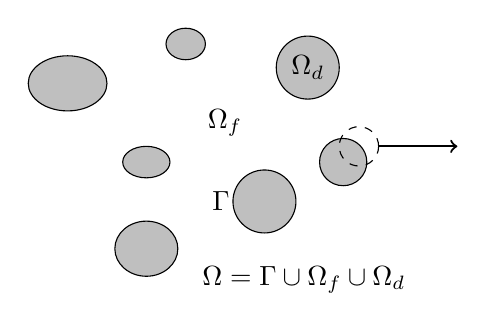
\begin{tikzpicture}
        \foreach \x/\y/\ra/\r in {
        1/3/0.2/0.25,
        2.55/2.7/0.4/0.4,
        0.5/0.4/0.35/0.4,
        2/1/0.4/0.4,
        3/1.5/0.3/0.3,
        0.5/1.5/0.2/0.3,
        -0.5/2.5/0.35/0.5}{
            \draw[fill=gray!50](\x,\y) ellipse(\r cm and \ra cm);
        }
        \draw[dashed](3.2,1.7)circle(0.25);
        % \draw[thick,->](3.2,1.7)++(0.1767,0.1767)--++(0.4,0.4)--++(1,0);
        \draw[thick,->](3.2,1.7)++(0.25,0)--++(1,0);
        \draw(2.55,2.7)node{$\Omega_d$};
        \draw(1.5,2)node{$\Omega_f$};
        \draw(1.45,1)node{$\Gamma$};
        \draw(2.5,0)node{$\Omega = \Gamma \cup \Omega_f \cup \Omega_d$};
        % \draw(2.5,-1)node{$\Gamma = \sum_\alpha \Gamma_\alpha$};
        % \draw(2.5,-0.5)node{$\Omega_2 = \sum_\alpha \Omega_\alpha$};
    \end{tikzpicture}
    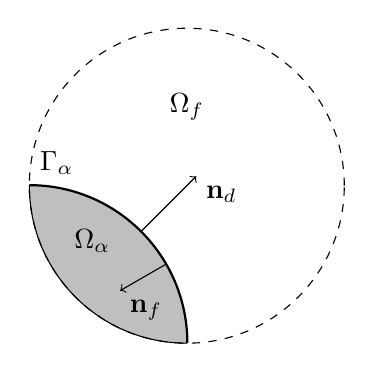
\begin{tikzpicture}%[scale = 0.9]
        \draw[very thick](0:2)arc(0:90:2)node[above right]{$\Gamma_\alpha$};
        \draw[fill=gray!50](0:2)arc(0:90:2)arc(180:270:2);
        \draw[dashed](2,2)circle(2);
        \draw[->](1.42,1.42)--++(0.7,0.7)node[below right]{$\textbf{n}_d$};
        \draw[->](1.73,1)--++(-0.577,-0.333)node[below right]{$\textbf{n}_f$};
        \draw(2,3)node{$\Omega_f$};
        \draw(0.8,1.3)node{$\Omega_\alpha$};
    \end{tikzpicture}
    \caption{Topology of dispersed two-phase flows.}%Domain definitions and scheme of the topology of dispersed two-phase flows.}
    \label{fig:Scheme}
\end{figure}

We consider a system consisting of two phases, separated by a sharp interface $\Gamma(t,\FF)$,
where $t$ represents the current time and $\FF$ a flow realization over a set of possible dispersed multiphase flow realization.  
A realization can be represented by a list of variables such as particle positions, velocities and other factors that provide a complete and unique description of the flow \citep{zhang2021ensemble}. %an initial flow configuration. 
%Further explanation about the concept of a flow realization will be provided later. 
%For now, it can be thought as an initial flow configuration. %Troughout this work we use the superscript `` $^0$ '' on a field to indicate that it is defined at the local non average level, which implies that it is a function of the flow configuration $\FF$, the position vector $\textbf{x}$, and the time $t$.
%More detail will be given later regarding the meaning of what is a flow realization. %we call the initial \textit{flow configuration}. 
%For now we may just think of it as an initial flow configuration.
%For now just think of it as a way to denote the dependence of the local functions such as $\Gamma(t,\FF)$ on the exact flow configuration. 
%In opposition to the averaged fields introduced in \ref{sec:avg_def} which will be defined as the average of these local functions over all the configurations $\FF$. 
The phase subdomains are labeled as $\Omega_f(t,\FF)$ and $\Omega_d(t,\FF)$, corresponding to the continuous (fluid) phase ($f$) and the dispersed phase ($d$), respectively (see \ref{fig:Scheme}). 
The complete domain, $\Omega$, is composed of the union of $\Omega_f$, $\Omega_d$, and $\Gamma$. To track the position of phase $k$ and the interfaces, we introduce the phase indicator function $\chi_k$ defined as follows

%Each phase subdomain is denoted as $\Omega_f(t,\FF)$ and $\Omega_d(t,\FF)$, representing the continuous or fluid phase ($f$) and the dispersed phase ($d$), respectively (refer to Figure \ref{fig:Scheme}).
%The entire domain, denoted as $\Omega$, is defined as the union of $\Omega_f$, $\Omega_d$, and $\Gamma$.
%To track the position of the phase indexed $k$ and the interfaces, we introduce the phase indicator function $\chi_k$ defined as
\begin{align}
    \chi_k(\textbf{x},t,\FF) =  \left\{
      \begin{tabular}{cc}
        $1 \;\text{if} \;\textbf{x} \in \Omega_k(t,\FF)$\\
        $0 \;\text{if} \;\textbf{x} \notin \Omega_k(t,\FF)$
      \end{tabular}
      \right.
      \text{for $k = f,d$}.
      \label{eq:PIF}
\end{align}
Additionally, we define $\Omega_\alpha(t, \FF)$ as the region occupied by particle $\alpha$ at time $t$ within the configuration $\FF$ (\ref{fig:Scheme}). The collective union of $\Omega_\alpha(t, \FF)$ for $\alpha = 1, \ldots, N$, where $N$ denotes the number of particles present in the flow, corresponds to $\Omega_d(t, \FF)$. Similarly, we assume that $\Gamma(t, \FF)$ can be partitioned into $N$ subregions, labeled $\Gamma_\alpha(t, \FF)$, each representing the surface of particle $\alpha$.

%Additionally, we define $\Omega_\alpha(t,\FF)$ as the domain delimited by the volume occupied by the particle labelled $\alpha$ at time $t$ and in the configuration $\FF$ (see \ref{fig:Scheme}). 
%The union of each $\Omega_\alpha(t,\FF)$ for $\alpha = 1,\ldots N$, assuming $N$ particles are present in the flow, is equivalent to $\Omega_d(t,\FF)$.
%Likewise, we suppose that $\Gamma(t,\FF)$ can be subdivided into $N$ subdomains denoted $\Gamma_\alpha(t,\FF)$, each of which represents the surface of the particle $\alpha$. 

\subsection{Topological equations}
Using the distribution formalism, one may show that $\chi_k(\textbf{x},t,\FF)$ obeys the following relations \citep{drew1983mathematical}. 
\begin{align}
    \pddt \chi_k
    + \textbf{u}_\Gamma^0 \cdot \grad \chi_k
    &= 0,
    \label{eq:dt_chi_k}\\
    \label{eq:grad_chi_k}
    \grad \chi_k
    &= - \delta_\Gamma \textbf{n}_k, 
\end{align}
where $\textbf{u}^0_\Gamma(\textbf{x},t,\FF)$ is the velocity of the interface and $\delta_\Gamma(\textbf{x},t,\FF)$ denotes the Dirac function localized on the interface, also called the interfacial indicator function \citep{drew1983mathematical,junqua2003}. 
More specifically the distribution $\delta_\Gamma$ is defined as \citep{appel2007}
\begin{equation}
<\delta_\Gamma,\varphi> =\int_{\Gamma} \varphi d\Gamma 
\label{eq:def_surf_distribution}
\end{equation}  
where $\varphi$ is a function with compact support. %in space-time
%\color{blue}
%a reformuler.
%\color{black}
In this work, we use the subscript $_\Gamma$ to denote any quantity inherently defined on the interfaces, such as $\textbf{u}_\Gamma^0(\textbf{x}, t, \FF)$ and $\delta_\Gamma(\textbf{x}, t, \FF)$. Additionally, we employ the superscript $^0$ on a field to indicate that it is defined at the local, non-averaged level, meaning it is a function of the flow configuration $\FF$, the position vector $\textbf{x}$, and time $t$. For clarity and readability, we omit the arguments $\FF$, $\textbf{x}$, and $t$ for any local function denoted by $^0$ (as well as for $\delta_\Gamma$ and $\chi_k$), as their dependence on $\textbf{x}$, $t$, and $\FF$ is implied.
%Throughout this work we employ the subscript $_\Gamma$ to indicate any quantity inherently defined on the interfaces, such as $\textbf{u}_\Gamma^0(\textbf{x},t,\FF)$ and $\delta_\Gamma(\textbf{x},t,\FF)$. 
%Furthermore, we use the superscript `` $^0$ '' on a field to indicate that it is defined at the local non average level, which implies that it is a function of the flow configuration $\FF$, the position vector $\textbf{x}$, and the time $t$. 
%For clarity and ease of reading purposes, we omit the arguments $\FF$, $\textbf{x}$ and $t$ for any local function denoted by a `` $^0$ '' (as well as for $\delta_\Gamma$ and $\chi_k$) as their dependence implicitly referring to $\textbf{x},t$ and $\FF$.

To derive a conservation equation for $\delta_\Gamma$, one can take the gradient of \ref{eq:dt_chi_k} and then compute the dot product of the resulting expression with $\textbf{n}_k$. This approach yields the following result \citep{marle1982macroscopic,drew1990,lhuillier2000bilan,junqua2003}
%One may obtain a conservation equation for $\delta_\Gamma$ by taking the gradient of \ref{eq:dt_chi_k} and then applying the dot product of the resulting expression with $\textbf{n}_k$. We obtain \citep{junqua2003,orlando2023evolutionevolution} %describe the evolution of $\delta_\Gamma$ we derive a first equation by taking the gradient of \ref{eq:dt_chi_k} and then applying the dot product of the resulting expression with $\textbf{n}_k$.

\begin{equation}
    \pddt \delta_\Gamma
    + \div [(\textbf{u}_\Gamma^0\cdot \textbf{n}) \textbf{n}\delta_\Gamma ]
    = (\textbf{u}_\Gamma^0 \cdot \textbf{n})(\div\textbf{n}) \delta_\Gamma ,
    \label{eq:dt_delta_I}
\end{equation} 
where we make use of the relation $\textbf{n}_k\cdot \pddt\textbf{n}_k= \frac{1}{2}\pddt(\textbf{n}_k\cdot \textbf{n}_k) = 0$. 
We did not specify the index of the normal $\textbf{n}$ in \ref{eq:dt_delta_I} to emphasize that this equation is independent of the index $k$. This is because $\textbf{n}$ appears twice in each term of this equation. 
Likewise, we will omit the index of the normal vector in subsequent discussions unless it is required. %For this reason, in the following, we will not specifcy the index of the normal when this it not necessary. %Furthermore, note that in  \ref{eq:dt_delta_I} and \ref{eq:grad_delta_I}.
Additionally, note that in \ref{eq:dt_delta_I} only the normal component of the surface velocity is present, and the term $\div \textbf{n}$ represents twice the mean curvature of the surface \citep{aris2012vectors}.  %\color{blue} 
A second equation is obtained by taking the gradient of the distribution $\delta_\Gamma $ (\ref{ap:delta_I}), namely, 
%With a slight abuse of notation the preceding relation may be rewritten as
%Multiplying the integrand by $\frac{n_{k}} \cdot \frac{n_{k}}$ and  we get 
%\begin{equation}
%<\frac{\partial}{\partial x_i}\delta_\Gamma ,\phi> = - \int_{\Gamma} \frac{\partial}{\partial x_i}\phi d\Gamma
%\end{equation}
%\color{black}
%A second equation is obtained by taking the gradient of the trivial relation $\delta_\Gamma  = \delta_\Gamma  \textbf{n}_k\cdot \textbf{n}_k$, resulting in
%. This yields, %\citep{morel2007surface,orlando2023evolution}, 
\begin{equation}
    \grad\delta_\Gamma  
    =   \grad (\textbf{n} \delta_\Gamma) \cdot \textbf{n}.
    \label{eq:grad_delta_I}
\end{equation}
\ref{eq:grad_delta_I} has been derived straightforwardly, yet it differs from the expression recently obtained by \citet{orlando2023evolution}.  The source of this discrepancy is unclear to the current authors. 
It might be due to differences in their notation, with their operator gradient potentially representing a normal derivative. 
%The source of this discrepancy is unclear to the current authors, but it may be related to discrepancy in their notation, their operator graident actually meaning normal derivative. %the definition of the gradient operator in \citet{orlando2023evolution}, which could be the normal derivative in their paper.
%Althoutgh, \ref{eq:grad_delta_I} has been derived straightforwardaly it is different from the expression recently derived by \citet{orlando2023evolution}. It is not clear to the present authors where does this difference comes from, although it might be related to the definition of the gradient operator in \citet{orlando2023evolution} which might be the normal derivative in his paper. 
%\ref{eq:grad_delta_I} has been derived straightforwardly in \ref{ap:delta_I}, yet it differs from the expression recently obtained by \citet{orlando2023}.  The source of this discrepancy is unclear to the current authors. It might be due to differences in their notation, with their operator gradient potentially representing a normal derivative.%The source of this discrepancy is unclear to the current authors, but it may be related to discrepancy in their notation, their operator graident actually meaning normal derivative. %the definition of the gradient operator in \citet{orlando2023}, which could be the normal derivative in their paper.
%Althoutgh, \ref{eq:grad_delta_I} has been derived straightforwardaly it is different from the expression recently derived by \citet{orlando2023}. It is not clear to the present authors where does this difference comes from, although it might be related to the definition of the gradient operator in \citet{orlando2023} which might be the normal derivative in his paper. 
%Remark that to derive \ref{eq:dt_delta_I} and \ref{eq:grad_delta_I} we have utilized the relations $\textbf{n}_k\cdot \pddt\textbf{n}_k= \frac{1}{2}\pddt(\textbf{n}_k\cdot \textbf{n}_k) = 0$ and $\grad \textbf{n}_k \cdot \textbf{n}_k =\frac{1}{2} \grad(\textbf{n}_k\cdot \textbf{n}_k) = 0$. 
\ref{eq:dt_chi_k}, \ref{eq:grad_chi_k}, \ref{eq:dt_delta_I} and \ref{eq:grad_delta_I}  are commonly referred to as the topological equations of two-phase flows.
These equations describe the spatiotemporal evolution of the interfaces topology.

\subsection{Local conservation equations}
\label{sec:local_eq}
We now introduce the local conservation laws that govern the fluid inside bulk phases (inside $\Omega_d$ and $\Omega_f$) and on the interfaces (on $\Gamma$). 
% \subsubsection{Generic formulation}
% We present generic conservation laws within the volumes and at the interfaces. 
Let $f_k^0$ denote a volumetric quantity of arbitrary tensorial order defined in $\Omega_k$.
Similarly, let $f_\Gamma^0$ represent an arbitrary surface property defined on $\Gamma$. 
Note that $f_\Gamma^0$ can be defined as a volumetric quantity integrated over the thickness of the interfaces \citet[Chapter 2]{ishii2010thermo}. 
Therefore, if $f_k^0$ has units $[x]$, then $f_I^0$ has the unit $[x.L]$, where $L$ is the unit of a length. 
The subscript $_{||}$ is used to denote the projection of a field onto the plane tangential to the surface $\Gamma$. Specifically, for an arbitrary quantity $\textbf{g}$ defined on $\Gamma$, its tangential projection is given by $\textbf{g}_{||} = \bm\delta_{||}\cdot \textbf{g}$ where $\bm\delta_{||} = (\bm\delta-\textbf{nn})$ is a tangential projection operator and $\bm\delta$ is the identity tensor. 
This definition also extends to the gradient operator, where $\gradI= \bm\delta _{||}\cdot \grad$ is referred to as the surface gradient operator. In addition we may define the surface divergence operator as $\gradI \cdot ()= (\bm\delta _{||}\cdot \grad)\cdot()$.

%We use the subscript  $_{||}$ to indicate the projection of a field onto the plane tangential to the surface $\Gamma$. Specifically, for an arbitrary quantity $\textbf{g}$ defined on $\Gamma$, we denote its tangential projection as $\textbf{g}_{||} = (\bm\delta-\textbf{nn})\cdot \textbf{g}$. The previous definition also applies to the divergence operator, meaning that $\gradI= (\bm\delta-\textbf{nn})\cdot \grad$ is referred to as the surface divergence operator. 

Following the strategy outlined in \citep{e2001mechanical,ishii2010thermo,bothe2022sharp}, the local conservation equations for $f_k^0$ and $f_\Gamma^0$ can be written as follows,
\begin{align}
    \label{eq:dt_f_k}
    \pddt f_k^0
    +\div \left(
        f_k^0\textbf{u}_k^0
        - \mathbf{\Phi}_k^0
        \right)
    &= 
    s_k^0
    & \text{ in } \Omega_k,&\\
    \pddt f_\Gamma^0 
    + f_\Gamma^0 (\textbf{u}_\Gamma^0 \cdot \textbf{n})(\div \textbf{n})
    +\divI
    (f_\Gamma^0 \textbf{u}_{\Gamma||}^0
        - \mathbf{\Phi}_{\Gamma||}^0 )
    &= 
    s_\Gamma^0
    - \Jump{
       f_k (\textbf{u}_\Gamma^0 - \textbf{u}_k^0)
       + \mathbf{\Phi}_k^0
    } 
    & \text{ on } \Gamma.&
    \label{eq:dt_f_I}
\end{align}
The tensors $\mathbf{\Phi}_k^0$ and $\mathbf{\Phi}_{\Gamma||}^0$ represent the non-convective fluxes corresponding to the quantities $f_k^0$ and $f_\Gamma^0$, respectively. Similarly, $s_k^0$ and $s_\Gamma^0$ are the source terms corresponding to the quantities $f_k^0$ and $f_\Gamma^0$, respectively. We assume that only the tangential component of the tensor $\mathbf{\Phi}_{\Gamma}^0$ plays a role in the surface balance equation \citep{bothe2022sharp}. 
% However, in certain specific scenarios, such as momentum transport along a membrane, the interface may exhibit resistance to bending. For further discussion on this topic, see \citet{jaensson2021}. 
% although in some very specific scenario for instance momentum tranport along a mebrane, the interface may resist bending. See for instance \citet{jaensson2019} for a discussion on the subject.
%. In some very specific scenario the interface may resist bending, see for instance Jaensson for a discussion on the subject.
%Note that $\mathbf{\Phi}_{\Gamma||}^0$ carries the $_{||}$ subscript which implies that only the tangential component of this tensor plays a role in the surface balance equation. Indeed we use the subscript  $_{||}$ to indicate the projection of a field onto the plane tangential to the surface $\Gamma$.  
%Thus, note that the diffusive flux $\bm\Phi_{I||}^0$ in \ref{eq:dt_f_I} is a quantity projected onto the tangential plane of $\Gamma$.
%This arises from the fact that at thermodynamic equilibrium the diffusive flux $\bm\Phi_{I||}^0$ exhibits solely tangential components.
%Indeed, in most of the cases the interfacial stress or heat fluxes, or mass fluxes.  
%Specifically, we can write \citep{nadim1996concise,bothe2022sharp}
%\begin{equation}
%    \bm\sigma_{I||}^0 = \left[\gamma + (\mu_{Id} -\mu_{Is}) \divI\textbf{u}_\Gamma^0\right] \bm\delta_{||}
%    +  \mu_{Is} \bm\delta_{||} \left[\grad_I\textbf{u}_\Gamma^0 + (\gradI \textbf{u}_\Gamma^0)^\dagger\right] \bm\delta_{||},
%    \label{eq:surface_fluxes}
%\end{equation}
%where $\mu_{Id}$ and $\mu_{Is}$ are the interfaces dilatational and shear viscosities, respectively, and $\gamma$ is the surface tension coefficient. 
%This observation holds significant implications for later analysis.
Consequently, the flux terms of the form $\divI[(\ldots)_{||}]$ in \ref{eq:dt_f_I} represent two-dimensional  convective and non-convective fluxes arising from tangential motions or diffusive processes at the interface.
Conversely, the term involving the local curvature $(\div \textbf{n})$ is related to the interface expansion or contraction resulting from the normal velocity of the interface $\textbf{u}_\Gamma^0\cdot \textbf{n}$. For practical uses, note that the advecting term in \ref{eq:dt_f_I} can be written in the more compact form $\divI(f_\Gamma^0 \textbf{u}_\Gamma^0)$. 
Indeed, one can show that $f_\Gamma^0 (\textbf{u}_\Gamma^0 \cdot \textbf{n})(\div \textbf{n})
+\divI(f_\Gamma^0 \textbf{u}_{I||}^0) = \divI(f_\Gamma^0 \textbf{u}_\Gamma^0)$, by noticing that $\textbf{n}\cdot\gradI(\ldots) = 0$ and $\divI\textbf{n} = \div\textbf{n}$ \citep{nadim1996concise}.
%Thus, the latter term is the consequence of the time-varying metric of the interface, while the former can be non-zero for a static interface $\Gamma$. 
In \ref{eq:dt_f_I} we have introduced the notation $\Jump{\ldots}$, where $\Jump{\ldots} = \sum_{k=1}^2 [\ldots] \cdot \textbf{n}_k$ signifies the jump across the interface. Thus, the last term on the right-hand side of \ref{eq:dt_f_I} represent a source of $f_\Gamma^0$ due to the discontinuity of bulk properties on either side of the interface. We also recognize a term related to mass transfer proportional to $(\textbf{u}_\Gamma - \textbf{u}_k)$. %$\rho_k^0 (\ldots) (\textbf{u}_\Gamma - \textbf{u}_k)$ where $(\ldots)$ refers to the quantity to be conserved. 
It is important to note that \ref{eq:dt_f_k} and \ref{eq:dt_f_I} are uniquely defined within the domains $\Omega_k$ and $\Gamma$, respectively.
Consequently, these equations are referred to as local conservation equations.



 


\subsection{The two-fluid formulation}
The phase indicator function $\chi_k$, and the Dirac delta function $\delta_\Gamma $, allow the extension of \ref{eq:dt_f_k} and \ref{eq:dt_f_I} to the entire flow domain $\Omega$. 
This extension is achieved by employing the methodology introduced by \citet{drew1983mathematical} and \citet{kataoka1986local} for the conserving laws inside the volume (\ref{eq:dt_f_k}).
The two-fluid formulation may be obtained by multiplying \ref{eq:dt_f_k} by $\chi_k$. 
Using \ref{eq:dt_chi_k} and \ref{eq:grad_chi_k} we obtain
\begin{equation}
    \pddt (\chi_k f_k^0)
    + \div (
        \chi_k f_k^0 \textbf{u}_k^0
        - \chi_k \mathbf{\Phi}_k^0 
        )
    = 
    \chi_k s_k^0
    + \delta_\Gamma \left[
        f_k^0
        \left(
            \textbf{u}_\Gamma^0
            - \textbf{u}_k^0
        \right)
        + \mathbf{\Phi}_k^0
    \right]
    \cdot \textbf{n}_k.
    \label{eq:dt_chi_k_f_k}
\end{equation}
This yields an equation defined over $\Omega$, to be solved for the quantity $\chi_k f_k^0$ instead of $f_k^0$. 
Moreover, in contrast to \ref{eq:dt_f_k} we observe the emergence of the interfacial term $ \delta_\Gamma [\ldots]$ on the right-hand side of \ref{eq:dt_chi_k_f_k}. 
To the best of the author's knowledge, the general form of the interfacial transport equation, expressed using the distribution formalism, has not yet been derived. However, some specific forms applicable to a given $f_i$ can be found in \citet{marle1982macroscopic} and  \citet{teigen2009}.
%To the best of the author knowledge the general form of the interfacial transport equation written using the distribution formalism has not been derived so far. Although some specific form valid for a given $f_i$ may be found in \citet{marle1982macroscopic,teigen2009}.%(citer Teigen et al. 2009 et Marle 1982)%for the conservation of mass exist in the litterature (citer Teigen et al. 2009 et Marle
%Likewise, multiplying \ref{eq:dt_f_I} by $\delta_\Gamma $ and making use of the topological equations (\ref{eq:dt_delta_I} and \ref{eq:grad_delta_I}) gives,
The derivation of this equation is straightforward but requires some algebra which is detailed in \ref{ap:interface_proof}. This yields%... As the derivation of \ref{eq:dt_delta_I_f_I} is not straightforward we provide intermediate steps in \ref{ap:interface_proof}. 
\begin{equation}
    \pddt (\delta_\Gamma f_\Gamma^0)  
    + \div (
        \delta_\Gamma  f_\Gamma^0 \textbf{u}_\Gamma^0
        - \delta_\Gamma  \mathbf{\Phi}_{\Gamma||}^0 
        )
    = 
    \delta_\Gamma s_\Gamma^0
    - \delta_\Gamma \Jump{
    f_k^0 (\textbf{u}_\Gamma^0 - \textbf{u}_k^0)
    + \mathbf{\Phi}_k^0},
    \label{eq:dt_delta_I_f_I}
\end{equation}
which corresponds to the conservation equation of $\delta_\Gamma f_\Gamma^0$, which is defined over $\Omega$.
Although \ref{eq:dt_f_I} and \ref{eq:dt_delta_I_f_I} appear similar in many respects, they possess a fundamental distinction: \ref{eq:dt_f_I} is defined exclusively on $\Gamma$, it is a two-dimensional partial differential equation with a time-dependent metric, whereas \ref{eq:dt_delta_I_f_I} is a three-dimensional partial differential equation. 
This distinction holds significant importance, as the formulation of \ref{eq:dt_delta_I_f_I} proves to be more practical for the numerical modeling of quantities on deformable interfaces \citep{teigen2009}. %methods %\citep{scorsim2021particle}. 
The set of equations formed by \ref{eq:dt_chi_k_f_k} for $k = f,d$ and the surface transport equation or \textit{jump condition} (\ref{eq:dt_delta_I_f_I}) is commonly known as the \textit{two-fluid} formulation of multiphase flows \citep{morel2015mathematical,tryggvason2011direct,drew1983mathematical,kataoka1986local}. 

According to \ref{eq:def_surf_distribution} the distribution  $\delta_\Gamma$ has the dimension of the inverse of a length, $[L^{-1}]$ \citep{appel2007}. 
Consequently, if the dimensionality of $f_k^0$ is assumed to be $[X]$, it follows that the dimensionality of $f_\Gamma^0$ must be $[X.L]$. Therefore , the product $\delta_\Gamma f_\Gamma^0$ carries the dimensionality $[X]$. %ensuring consistency in physical units.
Consequently, we can define a \textit{bulk} property $f^0$ as $f^0 = \sum_{k} \chi_k f_k^0 + \delta_\Gamma  f_\Gamma^0$ where $f^0$ represents any property of the flow of arbitrary tensorial order.
Then by summing \ref{eq:dt_chi_k_f_k} for $k=f,d$ and \ref{eq:dt_delta_I_f_I}, one obtain the \textit{bulk} formulation of multiphase flows, namely,%\textit{single-fluid} formulation of multiphase flows, namely,
\begin{equation}
   \pddt f^0
   + \div (
       f^0\textbf{u}^0
       -  \mathbf{\Phi}^0 
    )
   = s^0. 
   \label{eq:dt_f}
\end{equation}
where $f^0 \textbf{u}^0 = \sum_{k} \chi_k {f}_k^0\textbf{u}_k^0 + \delta_\Gamma  {f}_\Gamma^0\textbf{u}_\Gamma^0$, $\mathbf{\Phi}^0 = \sum_{k} \chi_k \mathbf{\Phi}_k^0 + \delta_\Gamma  \mathbf{\Phi}_\Gamma^0$ and $s^0 = \sum_{k} \chi_k s_k^0 + \delta_\Gamma  s_\Gamma^0$. 
In the literature, the \textit{single-fluid} formulation is characterized by summing only the quantities within the two phases, while the interfacial components are treated as source terms \citep{tryggvason2011direct,morel2015mathematical}.
%It should be noted that in the literature, the so called \textit{single-fluid} formulation is defined by summing only the quantities within the two phases while the interfacial components are treated as source terms in \ref{eq:dt_f} \citep{morel2015mathematical,tryggvason2011direct,drew1983mathematical}.  %with quantities as $f^0 = \sum_k \chi_k f_k^0$, while the interfacial components are treated as source terms in \ref{eq:dt_f} \citep{morel2015mathematical,tryggvason2011direct,drew1983mathematical}. 
Nevertheless, we want to point out here that our definition of $f^0$ yields a straightforward transport equation for $f^0$ thereby ensuring the consistency of the entire system of equations.



